\subsection{Red-Black Tree Implementation}
The c++ standard library contains a \textit{set} datatype as \texttt{std::set} which is implemented using a red-black tree so to ensure no errors in the implementation and to save some time, we decided to use that for our tests. This will also give the red-black tree a better chance at competing with our Van Emde Boas tree based search tree as we expect the standard library to be well optimized. We wrote a small class implementing Insert, Remove and Predecessor using a \texttt{std::set}. We also wrote a small class implementing the same, using either our vEB or bitsmart vEB tree as well as the min function to handle the case when there is no predecessor for our query in the interleaved test.

\subsection{Experiment Details}
Setup was much like in the previous heap tests, though the test themselves differed slightly.

\subsubsection{Test Types}
Four types of tests was done, where $n$ is the number of operations:
\begin{description}
\item[TestInserts] Tests the running time of Insert operations by measuring the time it takes to insert the $n$ elements $0$ to $n-1$.
\item[TestRemove] Tests the running time of Remove operations by measuring the time it takes to remove the $n$ elemens $0$ to $n-1$.
\item[TestPredecessor] Tests the running time of Predecessor operations by first filling the search tree with $\frac{n}{4}$ random~\footnote{because we use c++'s rand() with default seed, each test runs with the same input elements}, yet unique, elements and then calling the predecessor function on elements $0$ to $n-1$.
\item[TestInterleaved] Tests a somewhat closer to realistic scenario by first filling the search tree like in the TestPredecessor test and then $n$ times querying for the predecessor of a random element, removing it from the datastructure and inserting it again.
\end{description}

\subsection{Expectations}

In this second test we expect to see similar trends as in the first, with the Van Emde Boas trees being significantly faster than the Red-Black tree. In terms of memory, we expect the normal Van Emde Boas tree to use a very large chunk of memory, but hope that our bitsmart Van Emde Boas tree will use a constant \textit{small} amount of memory, hopefully less than the Red-Black tree at large data sizes.

\subsection{Data}
\subsubsection{Running Times}
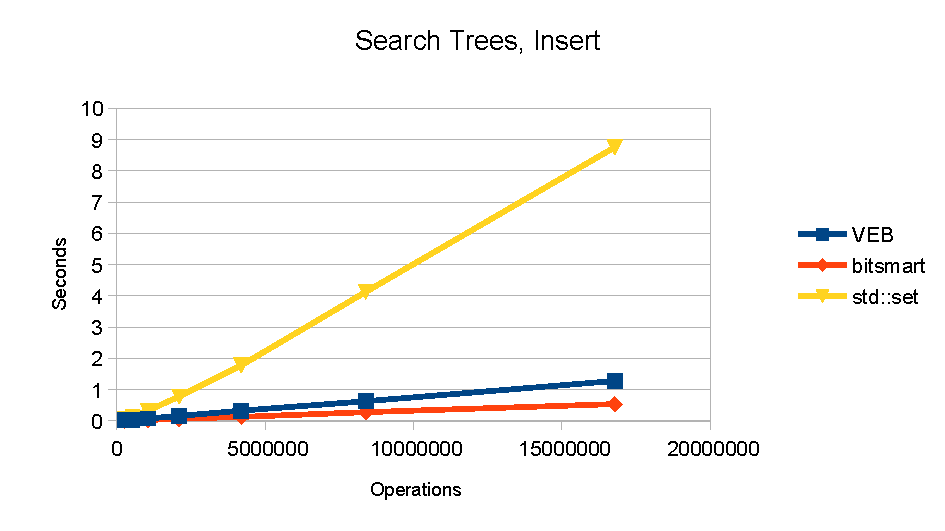
\includegraphics[width=\textwidth]{graphs/st_insert.pdf}
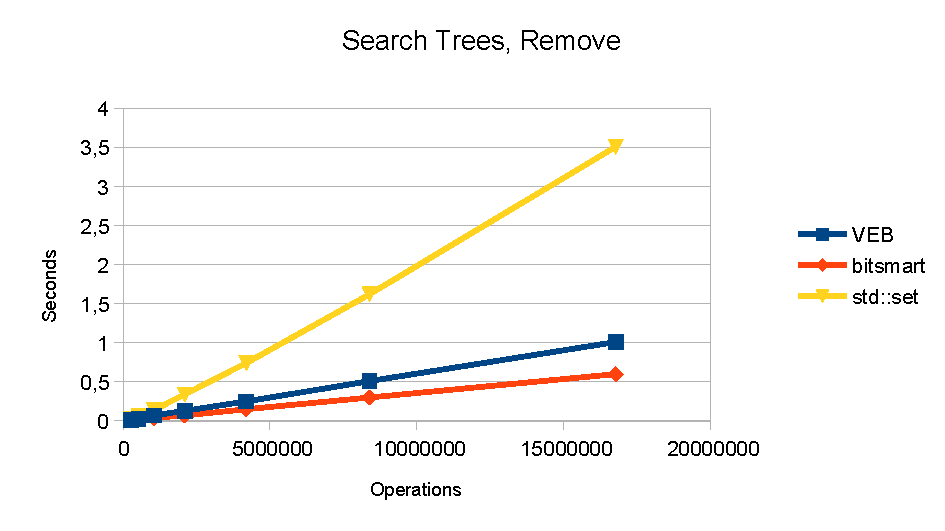
\includegraphics[width=\textwidth]{graphs/st_remove.pdf}
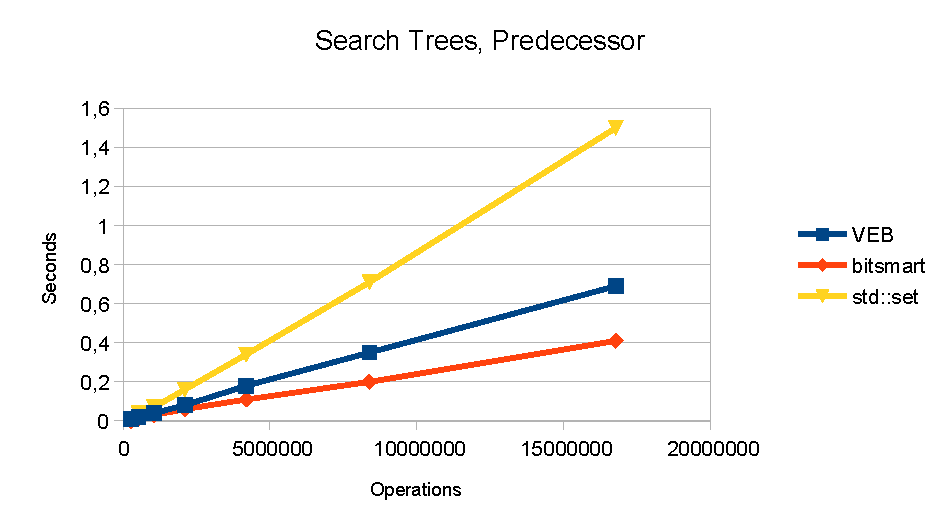
\includegraphics[width=\textwidth]{graphs/st_predecessor.pdf}
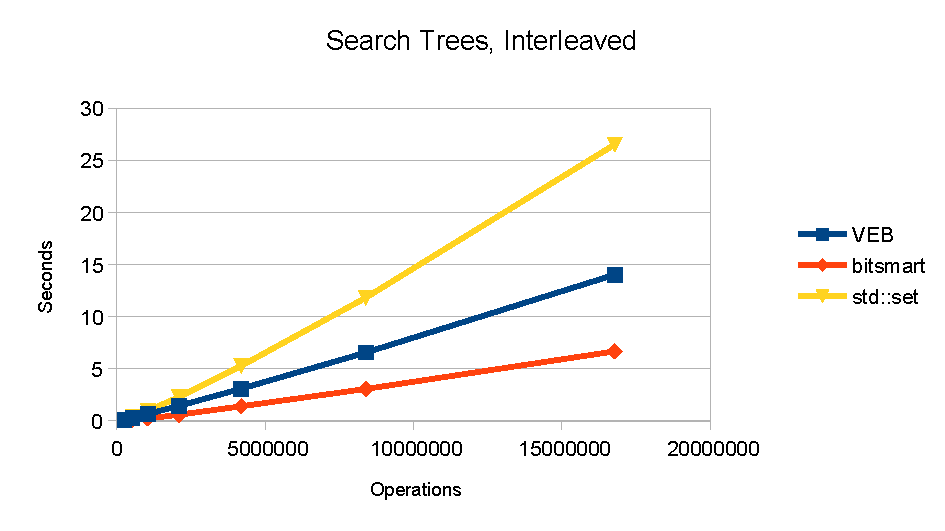
\includegraphics[width=\textwidth]{graphs/st_interleaved.pdf}

\subsubsection{Memory}
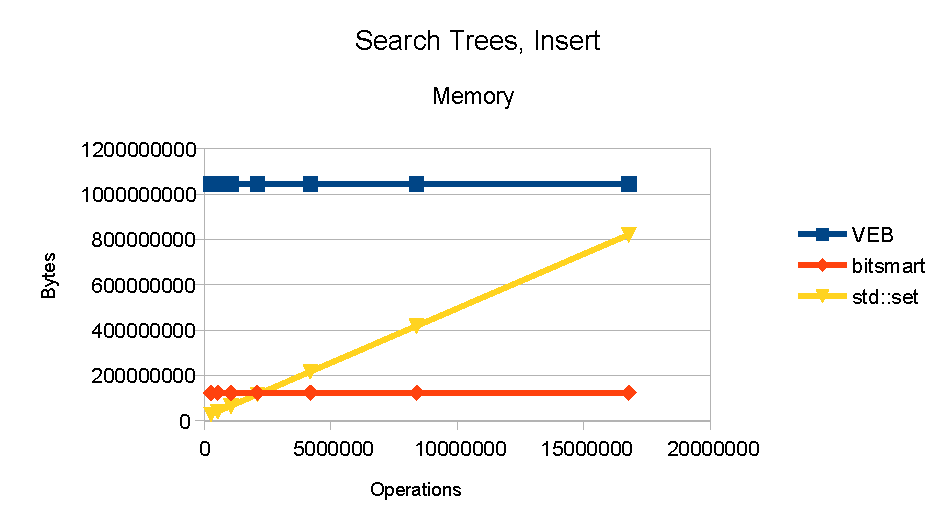
\includegraphics[width=\textwidth]{graphs/st_insert_memory.pdf}